%%%%%%%%%%%%%%%%%%%%%%%%%%%%%%%%%%%
%This is the LaTeX ARTICLE template for RSC journals
%Copyright The Royal Society of Chemistry 2016
%%%%%%%%%%%%%%%%%%%%%%%%%%%%%%%%%%%

\documentclass[twoside,twocolumn,9pt]{article}
\usepackage{extsizes}
\usepackage[super,sort&compress,comma]{natbib} 
\usepackage[version=3]{mhchem}
\usepackage[left=1.5cm, right=1.5cm, top=1.785cm, bottom=2.0cm]{geometry}
\usepackage{balance}
\usepackage{mathptmx}
\usepackage{sectsty}
\usepackage{graphicx} 
\usepackage{lastpage}
\usepackage[format=plain,justification=justified,singlelinecheck=false,font={stretch=1.125,small,sf},labelfont=bf,labelsep=space]{caption}
\usepackage{float}
\usepackage{fancyhdr}
\usepackage{fnpos}
\usepackage[english]{babel}
\addto{\captionsenglish}{%
  \renewcommand{\refname}{Notes and references}
}
\usepackage{array}
\usepackage{droidsans}
\usepackage{charter}
\usepackage[T1]{fontenc}
\usepackage[usenames,dvipsnames]{xcolor}
\usepackage{setspace}
\usepackage[compact]{titlesec}
\usepackage{hyperref}
%%%Please don't disable any packages in the preamble, as this may cause the template to display incorrectly.%%%

\usepackage{epstopdf}%This line makes .eps figures into .pdf - please comment out if not required.

\definecolor{cream}{RGB}{222,217,201}

\begin{document}

\pagestyle{fancy}
\thispagestyle{plain}
\fancypagestyle{plain}{
%%%HEADER%%%
\renewcommand{\headrulewidth}{0pt}
}
%%%END OF HEADER%%%

%%%PAGE SETUP - Please do not change any commands within this section%%%
\makeFNbottom
\makeatletter
\renewcommand\LARGE{\@setfontsize\LARGE{15pt}{17}}
\renewcommand\Large{\@setfontsize\Large{12pt}{14}}
\renewcommand\large{\@setfontsize\large{10pt}{12}}
\renewcommand\footnotesize{\@setfontsize\footnotesize{7pt}{10}}
\makeatother

\renewcommand{\thefootnote}{\fnsymbol{footnote}}
\renewcommand\footnoterule{\vspace*{1pt}% 
\color{cream}\hrule width 3.5in height 0.4pt \color{black}\vspace*{5pt}} 
\setcounter{secnumdepth}{5}

\makeatletter 
\renewcommand\@biblabel[1]{#1}            
\renewcommand\@makefntext[1]% 
{\noindent\makebox[0pt][r]{\@thefnmark\,}#1}
\makeatother 
\renewcommand{\figurename}{\small{Fig.}~}
\sectionfont{\sffamily\Large}
\subsectionfont{\normalsize}
\subsubsectionfont{\bf}
\setstretch{1.125} %In particular, please do not alter this line.
\setlength{\skip\footins}{0.8cm}
\setlength{\footnotesep}{0.25cm}
\setlength{\jot}{10pt}
\titlespacing*{\section}{0pt}{4pt}{4pt}
\titlespacing*{\subsection}{0pt}{15pt}{1pt}
%%%END OF PAGE SETUP%%%

%%%FOOTER%%%
\fancyfoot{}
\fancyfoot[LO,RE]{\vspace{-7.1pt}
\includegraphics[height=9pt]{head_foot/LF}}
\fancyfoot[CO]{\vspace{-7.1pt}\hspace{13.2cm}
\includegraphics{head_foot/RF}}
\fancyfoot[CE]{\vspace{-7.2pt}\hspace{-14.2cm}
\includegraphics{head_foot/RF}}
\fancyfoot[RO]{\footnotesize{\sffamily{1--\pageref{LastPage} ~\textbar  \hspace{2pt}\thepage}}}
\fancyfoot[LE]{\footnotesize{\sffamily{\thepage~\textbar\hspace{3.45cm} 1--\pageref{LastPage}}}}
\fancyhead{}
\renewcommand{\headrulewidth}{0pt} 
\renewcommand{\footrulewidth}{0pt}
\setlength{\arrayrulewidth}{1pt}
\setlength{\columnsep}{6.5mm}
\setlength\bibsep{1pt}
%%%END OF FOOTER%%%

%%%FIGURE SETUP - please do not change any commands within this section%%%
\makeatletter 
\newlength{\figrulesep} 
\setlength{\figrulesep}{0.5\textfloatsep} 

\newcommand{\topfigrule}{\vspace*{-1pt}% 
\noindent{\color{cream}\rule[-\figrulesep]{\columnwidth}{1.5pt}} }

\newcommand{\botfigrule}{\vspace*{-2pt}% 
\noindent{\color{cream}\rule[\figrulesep]{\columnwidth}{1.5pt}} }

\newcommand{\dblfigrule}{\vspace*{-1pt}% 
\noindent{\color{cream}\rule[-\figrulesep]{\textwidth}{1.5pt}} }

\makeatother
%%%END OF FIGURE SETUP%%%

%%%TITLE, AUTHORS AND ABSTRACT%%%
\twocolumn[
  \begin{@twocolumnfalse}
{
\includegraphics[height=30pt]{head_foot/SM}\hfill\raisebox{0pt}[0pt][0pt]{
\includegraphics[height=55pt]{head_foot/RSC_LOGO_CMYK}}\\[1ex]

\includegraphics[width=18.5cm]{head_foot/header_bar}}\par
\vspace{1em}
\sffamily
\begin{tabular}{m{4.5cm} p{13.5cm} }


\includegraphics{head_foot/DOI} & \noindent\LARGE{\textbf{Instabilities of ring rivulets: Impact of wettability gradients$^\dag$}} \\%Article title goes here instead of the text "This is the title"
\vspace{0.3cm} & \vspace{0.3cm} \\

 & \noindent\large{Stefan Zitz,\textit{$^{a}$} Johan Roenby\textit{$^{a}$}} \\%Author names go here instead of "Full name", etc.

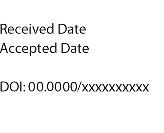
\includegraphics{head_foot/dates} & \noindent\normalsize{
Rivulets and droplets are naturally appearing shapes when small amounts of liquid are brought into contact with a partially wettable substrate.
Here we study, by the means of numerical simulations, the stability of a ring-rivulet placed on a solid substrate.
First we consider a ring-rivulet on a uniform substrate, similar to the work of Nguyen \textit{et al. Langmuir}, 2012, \textbf{28}, 13960-13967.
We then consider different kinds of patterning and show that they not only affect the stability but also the morphology.
Thus making it possible to turn ring rivulets which would break up into droplets into collapsing single droplet.} \\%The abstrast goes here instead of the text "The abstract should be..."

\end{tabular}

 \end{@twocolumnfalse} \vspace{0.6cm}

  ]
%%%END OF TITLE, AUTHORS AND ABSTRACT%%%

%%%FONT SETUP - please do not change any commands within this section
\renewcommand*\rmdefault{bch}\normalfont\upshape
\rmfamily
\section*{}
\vspace{-1cm}


%%%FOOTNOTES%%%

\footnotetext{\textit{$^{a}$~IMFUFA, Department of Science and Environment, Roskilde University, Postbox 260, 4000 Roskilde, DK. Tel: +45 2993 1923; E-mail: johan@ruc.dk}}
% \footnotetext{\textit{$^{b}$~Address, Address, Town, Country. }}

%Please use \dag to cite the ESI in the main text of the article.
%If you article does not have ESI please remove the the \dag symbol from the title and the footnotetext below.
\footnotetext{\dag~Electronic Supplementary Information (ESI) available: [details of any supplementary information available should be included here]. See DOI: 10.1039/cXsm00000x/}
%additional addresses can be cited as above using the lower-case letters, c, d, e... If all authors are from the same address, no letter is required

\footnotetext{\ddag~Additional footnotes to the title and authors can be included \textit{e.g.}\ `Present address:' or `These authors contributed equally to this work' as above using the symbols: \ddag, \textsection, and \P. Please place the appropriate symbol next to the author's name and include a \texttt{\textbackslash footnotetext} entry in the the correct place in the list.}


%%%END OF FOOTNOTES%%%

%%%MAIN TEXT%%%%
\section{Introduction}
\label{sec:intro}
Thin films and droplets play in an important role in our everyday life.


The outline of the paper is as follows

\section{Simulation method}
\label{sec:method}
For the time resolved simulations of a thin liquid ring-rivulet we use a recently developed lattice Boltzmann method (LBM) for thin films~\cite{zitzLatticeBoltzmannMethod2019, zitzSwalbeJlLattice2022}. 
Here we just give a short introduction into the method and highlight the relevant modelling approximations.
The thin film model is build on a class of LBMs originally proposed for shallow water systems~\cite{} 
\begin{equation}\label{eq:LBE}
\begin{split}
&f_l(\mathbf{x}+\mathbf{c}^{(l)}\Delta t,t+\Delta t) = \\
&(1 - \omega) f_l(\mathbf{x},t) + \omega f_l^{(eq)}(\mathbf{x},t) + w_l \frac{\Delta t}{c_s^2} \mathbf{c}^{(l)} \cdot \mathbf{F}_{\mbox{\tiny{tot}}},
\end{split}
\end{equation}
where $l$ labels the lattice velocities $\mathbf{c}_l$ and runs from $0$ to $Q-1$, with $Q$ being the number of velocities characterizing the scheme.
Algorithmically, this equation can be seen as made up of two steps. 
A {\it local collision} step where the $f_l(\mathbf{x},t)$ ``relax'' towards the local equilibrium distributions $f^{(eq)}_l(\mathbf{x},t)$ with rate  
$\omega = \Delta t/\tau$ (where $\tau$, the relaxation time, is proportional to the kinematic viscosity $\nu$): the distribution functions are substituted by their weighted average (with weights $\omega$ and $1-\omega$) with the equilibria, with an added so-called "source" term (the last term on the right hand side of Eq. (\ref{eq:LBE})), when a force is present. 
A {\it non-local streaming} step where the updated distribution functions are scattered to the nearest neighbouring sites. 
The parameters $c_s$ (the lattice speed of sound) and $w_l$ (the so called "weights")
depend on the geometry of the lattice and are determined under suitable constraints on the form of the tensorial moments in the lattice velocities up to fourth order~\cite{krugerLatticeBoltzmannMethod2017}.


\subsection{Initial conditions}
\begin{figure}
\centering
  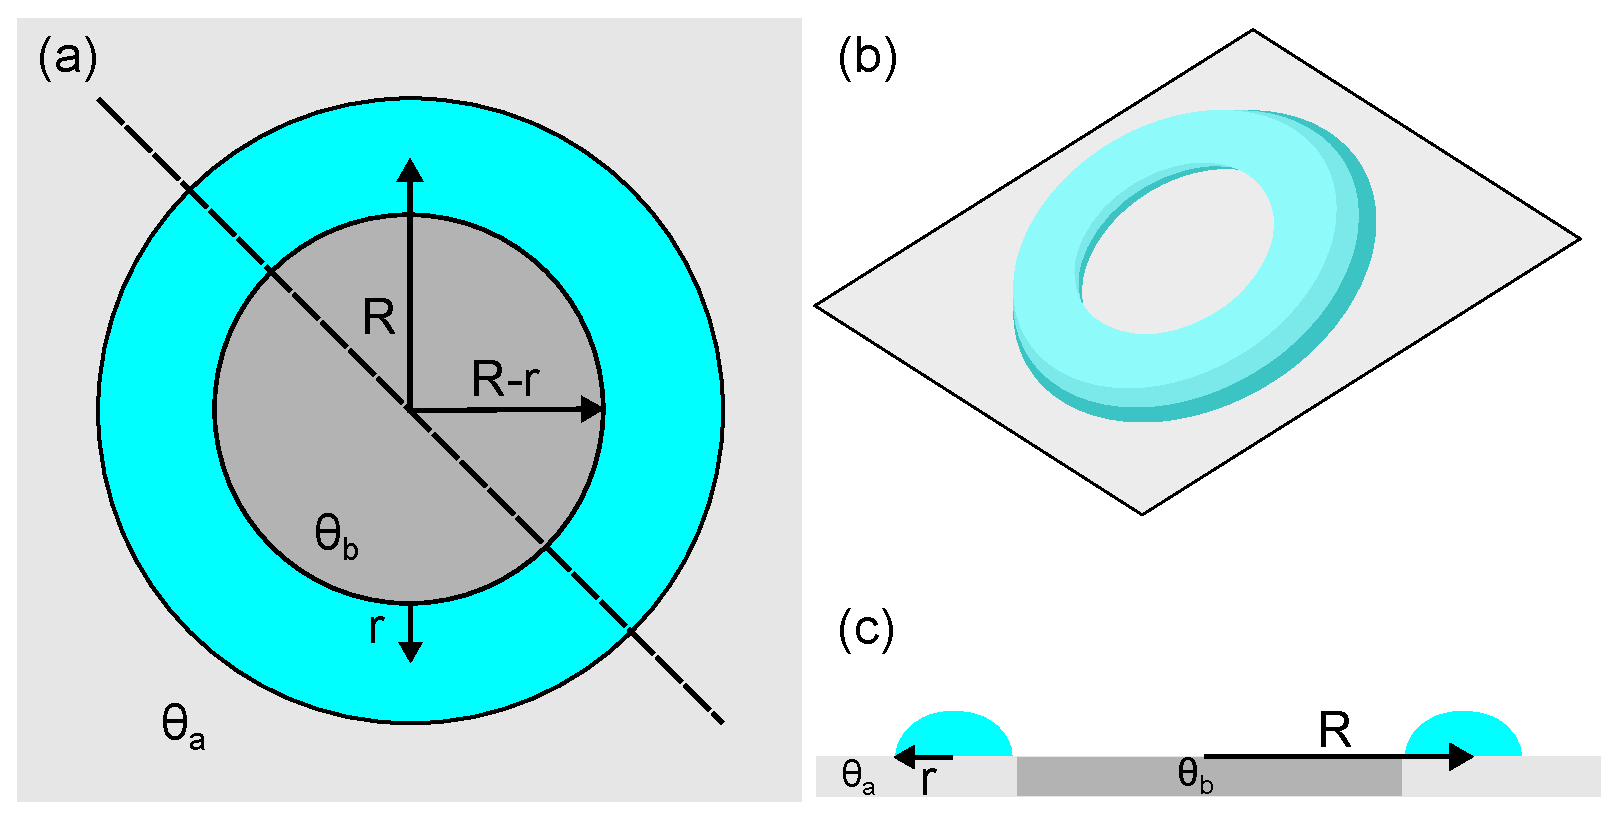
\includegraphics[width=0.45\textwidth]{ringrivulet_shema}
  \caption{Schematic setup of our initial conditions. In (a) we show the top view where $R$ and $r$ are the two different radii and $\theta_a$ and $\theta_b$ can be different contact angles. 
  In (b) we show an isometric view of the initial condition.
  By cutting along the dashed line in (a) we get the side view of (c).}
  \label{fgr:ringschema}
\end{figure}

The initial thickness profile $h(x,y)$ of the film at $t=0$ is set by an implicit equation for a torus with radial symmetry along the z-axis and is given by
\begin{equation}\label{eq:torus}
    h_t(x,y) = \sqrt{r^2 - \left(R-\xi\right)^2},
\end{equation}
where $\xi = \sqrt{(x-x_0)^2+(y-y_0)^2}$, $R$ is the major radius and $r$ is the minor radius of the torus.
The center of the torus is at $(x_0,y_0)$ and $h_t$ is the height of the torus.
We only consider the upper half with $h<0$ as shown in Fig.~\ref{fgr:ringschema}. 
The resulting fluid structure is a half-torus with $90^{\circ}$ contact angle.
This contact angle violates the long wave approximation $\theta \ll 1$, therefore we perform another cut to a smaller contact angle using
\begin{equation}
    h(x,y,t=0) = h_t(x,y) - r\cos(\theta)
\end{equation}
and set all $h < 0$ to $h = h_{\ast}$ which is the thickness of the precursor film.

Our main interest is focused on the impact of a pattern on the evolution of the ring-rivulet. 
As indicated in Fig.~\ref{fgr:ringschema} we use different contact angle configurations $\theta(x,y)$.
First we use 
\begin{equation}
    \theta(x,y) = \theta_0,
\end{equation}
where $\theta_0$ is a constant.
Next we consider a banded case, where the ring-rivulet has the same contact angle as its immediate surrounding and the rest of the substrate has a higher contact angle
\begin{equation}
    \theta(r_i) =\begin{cases}
        \theta_a,\quad \text{if}~h(\xi\pm \delta\xi) > 0\\
        \theta_b,\quad \text{else}
    \end{cases}.
\end{equation}
The addition of $\delta\xi$ widens the band and allow the ring-rivulet to contract a bit.  
Lastly, we consider a linear wettability gradient with decreasing contact angle towards the middle
\begin{equation}
    \theta(\xi) = \frac{\theta_{max}-\theta_{min}}{R} \xi + \theta_{min},
\end{equation}
where $\theta_{max}, \theta_{min}$ are the maximal, minimal contact angle respectively.

\section{Dynamics of ring rivulets}
\label{sec:dynamics}

The \texttt{mhchem} package can also be used so that formulae are easy to input: \texttt{\textbackslash ce\{H2SO4\}} gives \ce{H2SO4}. 

For footnotes in the main text of the article please number the footnotes to avoid duplicate symbols. \textit{e.g.}\ \texttt{\textbackslash footnote[num]\{your text\}}. The corresponding author $\ast$ counts as footnote 1, ESI as footnote 2, \textit{e.g.}\ if there is no ESI, please start at [num]=[2], if ESI is cited in the title please start at [num]=[3] \textit{etc.} Please also cite the ESI within the main body of the text using \dag. For the reference section, the style file \texttt{rsc.bst} can be used to generate the correct reference style.

\section{Conclusions}
The conclusions section should come in this section at the end of the article, before the Conflicts of interest statement.

\section*{Author Contributions}
We strongly encourage authors to include author contributions and recommend using \href{https://casrai.org/credit/}{CRediT} for standardised contribution descriptions. Please refer to our general \href{https://www.rsc.org/journals-books-databases/journal-authors-reviewers/author-responsibilities/}{author guidelines} for more information about authorship.

\section*{Conflicts of interest}
In accordance with our policy on \href{https://www.rsc.org/journals-books-databases/journal-authors-reviewers/author-responsibilities/#code-of-conduct}{Conflicts of interest} please ensure that a conflicts of interest statement is included in your manuscript here.  Please note that this statement is required for all submitted manuscripts.  If no conflicts exist, please state that ``There are no conflicts to declare''.

\section*{Acknowledgements}
The authors acknowledge financial support from the Independent Research Fund Denmark through a DFF Sapere Aude Research Leader grant (grant number 9063-00018B).

%%%END OF MAIN TEXT%%%

%The \balance command can be used to balance the columns on the final page if desired. It should be placed anywhere within the first column of the last page.

\balance

%If notes are included in your references you can change the title from 'References' to 'Notes and references' using the following command:
%\renewcommand\refname{Notes and references}

%%%REFERENCES%%%
\bibliography{rsc} %You need to replace "rsc" on this line with the name of your .bib file
\bibliographystyle{rsc} %the RSC's .bst file

\end{document}
